 \begin{figure*}[t]
\begin{center}
	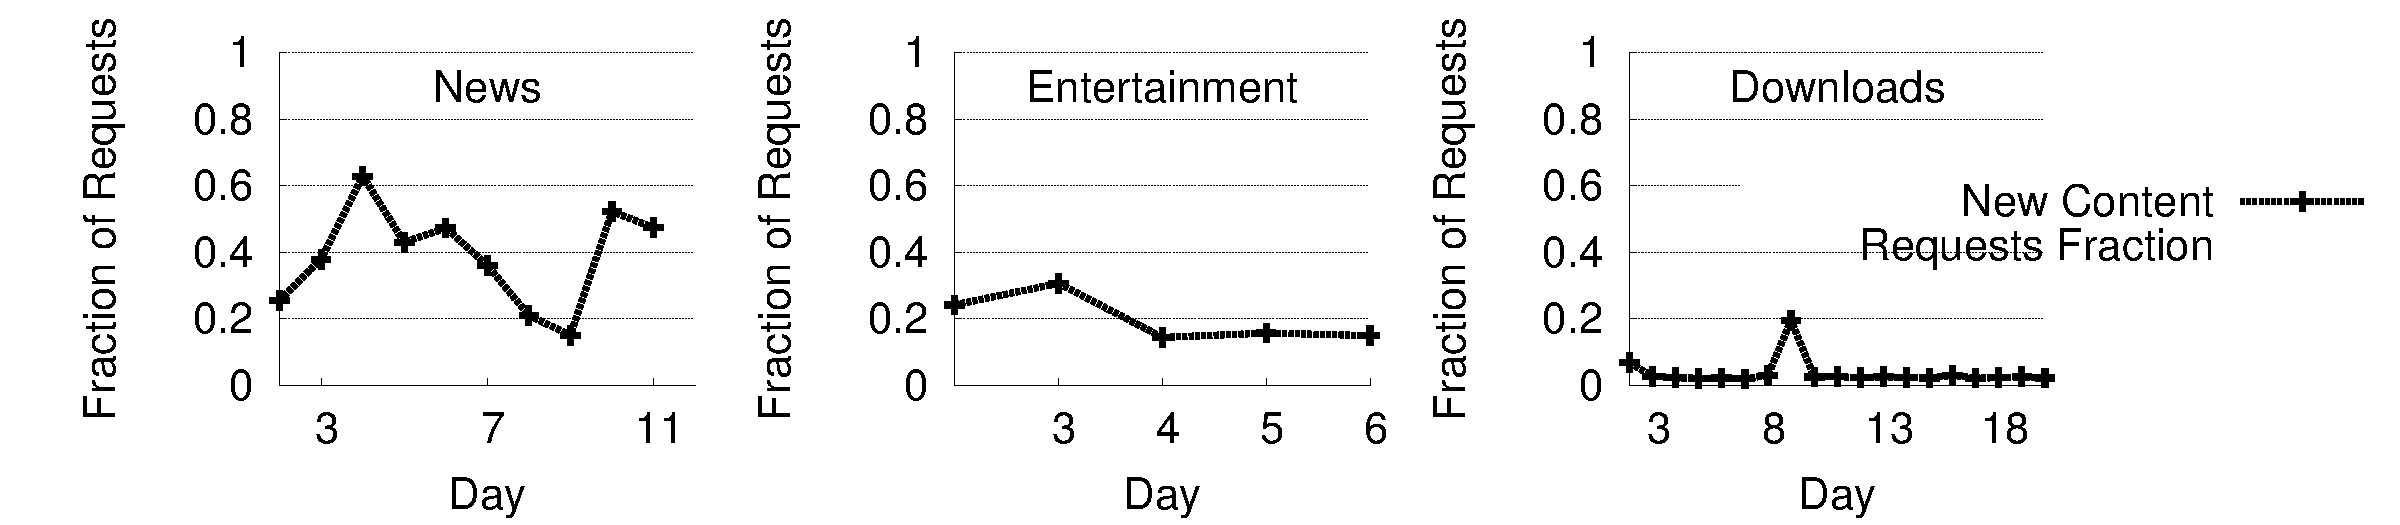
\includegraphics[scale=0.4]{graphSet1/akamaidata/churn.pdf}
\end{center}
\vspace{-0.3in}
\caption{News and entertainment have a significant fraction of requests for new content on all days. Downloads has a small fraction of requests for new content on all days, except one.}
\vspace{-0.25in}
\label{fig:akamaichurn}
\end{figure*}


\section{Akamai CDN traces}
\label{sec:dataset}
To conduct a realistic simulation of end-users accessing content on an  NCDN, we collected extensive traces of video and download traffic from Akamai as described below.
% We collected traces for the two major sources of CDN traffic that we describe in turn.

%Then, we used the topologies for two networks:  Abilene   and AT\&T  as described in Section \ref{sec:topology}. 

 %This facilitated combining the CDN content access logs with the network topology information to derive realistic simulations.

%We used a trace of users content requests from one of world's largest CDNs (described in Section \ref{sec:cdntrace}). We also experimented with synthetic traces of users content requests generated based on traffic matrices of two ISPs including a Tier-1 ISP (described in Section \ref{sec:isptrace}).




\eat
{
 \begin{figure*}
\begin{center}
\subfigure[News Trace]{
	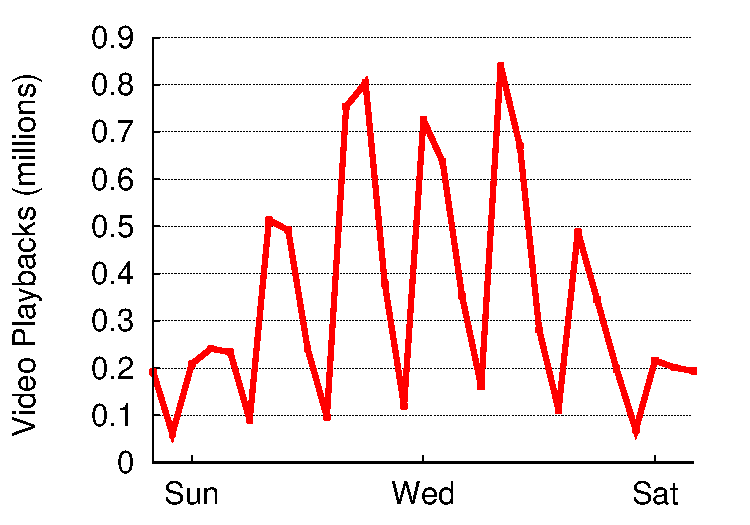
\includegraphics[scale=0.4]{graphSet1/akamaidata/NewsRequests.pdf}
\label{fig:news}}
\subfigure[Entertainement Trace]{
	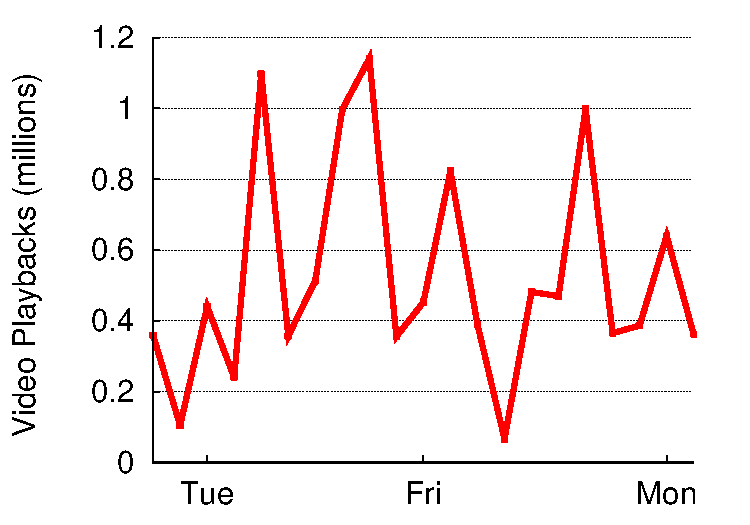
\includegraphics[scale=0.4]{graphSet1/akamaidata/TVRequests.pdf}
\label{fig:entertainment}}
\subfigure[Downloads Trace]{
	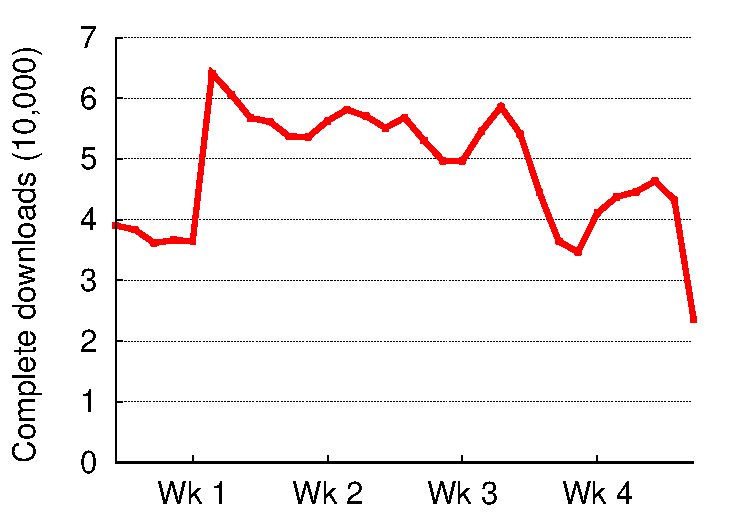
\includegraphics[scale=0.4]{graphSet1/akamaidata/SoftwareRequests.pdf}
\label{fig:downloadnumber}}
\end{center}
\caption{Number of videos played every 6 hours in the news trace (Figure \ref{fig:news}) and  the entertainment trace (Figure \ref{fig:entertainment}).  Figure \ref{fig:downloadnumber} shows the number of completed downloads on each day for the downloads trace. }
\label{fig:akamaistats}
\end{figure*}
}



\label{sec:CDNtraces}


{\bf Video traces.} Videos are the primary source of traffic on a CDN and are growing at a rapid rate \cite{nielsen-video-growth,cisco-videogrowth}. %In addition, many NCDNs are likely to be disproportionately focused on video due to the attractive business model of Telcos delivering on-demand video to their subscribers \cite{fios}.  
Our video trace consists of actual end-users accessing on-demand videos on the Akamai network over multiple days. To make the traces as representative as possible, we chose content providers with a whole range of business models, including major television networks, news outlets, and movie portals. The videos in our traces include a range of video types from  short-duration video (less than 10 mins) such as news clips to longer duration (30 min to 120 min) entertainment videos representing TV shows and movies. In all, our traces represent a nontrivial fraction of the overall traffic on Akamai's media network and accounted for a total of 27 million playbacks of over 85000 videos, 738  TBytes of traffic, served  to 6.59 million unique end-users around the US. Since we only had US-based network topologies with accurate link capacity information, we restricted ourselves to US-based traffic.

We collect two sets of video traces called  \emph{news trace} and \emph{entertainment trace} respectively.  The news trace was collected from a leading news outlet for an 11-day period in Sept 2011, and consists mostly of news video clips, but also includes a small fraction of news TV shows.  The entertainment trace was collected for a 6 day period in January 2012, and includes a variety of videos including TV shows, clips of TV shows,  movies and movie trailers from three major content providers.


%We collected two sets of video traces called  \emph{news trace} and \emph{entertainment trace} respectively.  News trace was collected from a leading news outlet for an 11-day period in Sept 2011. The videos in this trace consist mostly of news video clips, but also include a small fraction of news TV shows. Entertainment trace consists of content from three major content providers for a 6 day period in January 2012.   This trace includes a variety of videos including TV shows, clips of TV shows,  movies and movie trailers. 

%We call the second dataset   \emph{entertainment trace}. 

%We show the number of video playbacks  reported every 6 hours for subset of the news trace and the entertainment trace in Figure \ref{fig:akamaistats}.  

The trace collection mechanism utilized a plugin embedded in the media player that is capable of reporting (anonymized) video playback information. Our traces include a single log entry for each  playback and provides time of access, user id, the location of the user (unique id, city, state, country, latitude, and longitude), the url of the content, the content provider, the total length of the video (in time and bytes), the number of bytes actually downloaded, the playback duration, and the average bitrate over the playback session. 


{\bf Downloads traces.} The second largest traffic contributor in a CDN is  downloads of large files over HTTP. These include software and security updates,  e.g., Microsoft's Windows or Symantec's security updates, as well as music, books, movies, etc.. The large file downloads at Akamai typically use a client-side software called the download manager \cite{akamai-overview}. We collect extensive and  anonymized access data reported from the download manager using Akamai's NetSession interface \cite{netsessions} for a large fraction of content providers for a period of a month (December 2010). Our traces represent a nontrivial fraction of the overall US-based traffic on Akamai's downloads network  and accounted for a total of 1.2 million downloads, 717 TBytes of traffic, served to 0.62 million unique end-users around the US. Our traces provide a single log entry for each download and provide time of access, user id, location of the user (city, state, country, latitude, and longitude), the url identifier of the content, content provider, bytes downloaded, and file size.  

%We show the number of completed downloads on each day of the trace in Figure \ref{fig:downloadnumber}.
Figure \ref{fig:akamaichurn} shows the fraction of requests for new content published each day relative to the previous day for news, entertainment, and downloads traces. The news trace has up to 63\% requests due to new content because the latest news clips generated each day are the most popular videos on the website. The entertainment trace also has up to 31\% requests each day due to new content such as  new episodes of TV shows, and the previews of upcoming TV shows. The downloads trace has only 2-3\% requests due to new content on a typical day. However, on the 9th day of the trace major software updates were released, which were downloaded on the same day by a large number of users. Hence, nearly 20\% requests on that day were for new content. The fraction of requests for new content impacts the performance of \planned\ placement strategies as we show Section \ref{sec:ncdn-eval}.

%The x-axis shows the day of trace and the y-axis shows the fraction of requests (or traffic) for content published on that day. 

%The fraction of requests for new content impacts the performance of demand-aware placement strategies as we show in Section \ref{sec:eval}.

%Figure \ref{akamaichurn} shows 



%overall trace description
%We obtained two sets of traces consisting of logs of users' video playback  from one of the largest CDNs in the world. First trace is for short duration video content (less than 10 minutes), e.g. news clips,   and the second trace is for longer duration video  (30 min to 120 min), e. g., TV shows and movies. The short video trace is for a 10 day period in 2011 and the long video trace is for a 3 day period in 2011. From now on, we refer to these traces as CDN-SV (short videos) and CDN-LV (long videos).

% what does the log contain
%Each log entry tells us the location of the user, the time of access and the content being
% accessed.  A log entry also reports the number of bytes downloaded from CDN server to the client during the session  and the average bit rate of the video played. In addition, we know the duration of each video. 


% fraction of video downloaded
%Data set has information about the fraction of video downloaded by each user. we  assume user watched the duration video downloaded (though user would have actually watched less than the  downloaded video, the actual downloaded video depends on the implementation of video player).
%Our traces showed that a huge fraction of users downloaded much less than 100\% of video. In fact, 70\% of users downloaded less than 10\% of the video.
%We noticed that several related studies on Video-On-Demand content placement have not considered the fraction of video downloaded within their framework. 





 
%Each PoP (i.e., node)  of the NCDN has a deployment of content servers as shown in Figure~\ref{fig:NCNDArch}. We model the amount of storage available at each node as it is most relevant for our simulation and do not model other server resources such as CPU. Further, we assume that the storage is provisioned in a homogenous fashion with each node having the same amount. Heterogenous storage distribution is an easy future extension. 


%\noindent\textbf{bit rates and file sizes}
%Typically video is stored as well as played at multiple bit rates. We make a simplifying assumption that each video is stored and played at only one bit rate, which is the maximum bit rate of each  video from our trace. This also helps us determine the disk space needed to store the video. Since the duration of the video is independent of the bit rate, the disk space for each video is equal to   duration of video times the bit rate for each video.

%\noindent\textbf{Popularity distribution of content}
%For each trace, we need to find out the popularity distribution from trace. Network state is updated once in every epoch using TE scheme algorithm, the epoch length  is a parameter,  Every epoch , we update the content placement, based on popularity in the previous interval. The popularity for a content at a node is the number of requests for a content times the size of the content

%\noindent\textbf{Selecting popular content from trace}
%To select which content to place in the network out of all the content, we use thumb rules depending on average size of content. We keep a threshold of 10 accesses for short form videos and a threshold of 3 accesses for long form videos. 


%\noindent\textbf{Scaling link capacities}
%Since each of our datasets only consists of data from one client of a CDN, the aggregate traffic is a fraction of the total demand. hence we scale the network links to 1/10th of capacity so that MLU values resemble those found in ISP networks today.

%\noindent\textbf{Periodicity of traffic engineering}
%Epoch length is 1 day. This is derived from time scales at which traffic engineering is done today. That is content placement and routing are updated once a day based on previous day traces.


%\subsection{ISP Traffic Matrix Based Synthetic Traces}
%\label{sec:isptrace}

%We experimented with following ISP topologies and traffic matrix dataset  Abilene, and  a Tier-1 US ISP. From each dataset we randomly selected 10 traffic matrices for experiments.

%\noindent\textbf{ISP Topologies and Traffic Matrices:} 

%\noindent\textbf{Traffic Matrices:}
%We assumed that the total traffic demand at each node follows a gravity model, i.e., the traffic demand at a node is proportional to the sum of incoming link capacities at the node.

%\noindent\textbf{Number of unique content:}
%The number of unique pieces of content in our experiments is  1000 for all experiments. The number of content in the library of major service provides can possibly be an order of magnitude larger. But, solving for these equations with our current experiment setup does not complete even in three hours for each linear program with 10000 pieces of content.

%This number is likely to be an order of magnitude higher for content in an actual ISP network. But, optimally solving the linear programs is practically infeasible for those linear programs.

% times the number of nodes, i.e., there are 100 unique pieces of content in a 10 node network.

%\noindent\textbf{Content popularity distribution:}
%The traffic demand  for a content follows a Zipf distribution with parameter 1.5.   The number of requests for the most and least popular content differs by approximately three orders of magnitude.  We cut-off the distribution at the start to remove disproportionately high demand for highest ranked content in the Zipf distribution. For this, we assigned the number of requests for the top 1/10th of the most popular  pieces of content equal to the traffic demand for the content ranked  1/10th most popular content according to Zipf distribution.

%\noindent\textbf{Content popularity distribution across nodes:}
%We assume two types of content which differ in their distribution of popularity in the network - global popularity content and local popularity content. For a content with global popularity, the demand at a node  is proportional to the total traffic demand at that node. A locally popular content has all its demand at a randomly chosen node and its neighbors. By default, we experiment with 75\% content having a global popularity and 25\% having local popularity.


%\noindent\textbf{Content size distribution:}
%The size of the content in the network follows a Zipf distribution with parameter 1.  The values of 10\% biggest files are set to 1000 MB, in
%The size of the largest content is 1000 MB and the smallest content is  100 MB.  
%The sizes of the largest and smallest content differing by one order of magnitude.

%\noindent\textbf{Correlation between content size and its popularity:}
%We assume no correlation between content size and its popularity. A content is randomly assigned a popularity taken from the Zipf distribution of content popularity.

%\noindent\textbf{Replication Factor:} For each experiment, we choose a replication factor $k > 1$ and $k < $(Number of nodes). 

%\noindent\textbf{Storage at each PoP:}
%The storage in the network is assumed to be equal at all nodes. The sum of storage space at all nodes at all nodes is equal to the sum of the sizes of all content times the replication factor given.


